\documentclass{article}
\usepackage[margin=1in]{geometry}
\usepackage[T1]{fontenc}
\usepackage[utf8]{inputenc}
\usepackage{graphicx}
\usepackage{hyperref}
\usepackage{enumitem}
\begin{document}

\section*{SilverTorch: A Unified Model-based System to Democratize Large-Scale Recommendation on GPUs (2025)}
\textbf{arXiv:2511.14881v1 (cs.IR), 18 Nov 2025.}\\
\textbf{Verified PDF:} \url{https://arxiv.org/pdf/2511.14881.pdf}

\subsection*{Challenges}
\begin{itemize}[leftmargin=1.5em]
  \item \textbf{Service-based recommendation stacks are fragmented.} Production retrieval typically splits user towers, ANN indexing, feature filtering, caches, and rerankers across separate services. The paper argues this creates client-side orchestration complexity, communication overhead, and version inconsistency between model snapshots and indexes.
  \item \textbf{CPU-centric ANN + filtering bottleneck large-scale retrieval.} Industrial systems must search 10--100M items, often returning tens of thousands of candidates for downstream scoring. Existing CPU-based ANN/filtering pipelines are expensive and hard to scale for richer retrieval models; common GPU ANN systems also cap topk/probe settings in ways that do not fit recommendation workloads.
  \item \textbf{More accurate retrieval models are difficult to serve online.} Learned similarities, multi-task retrieval, and early-stage ranking need more computation than plain dot-product retrieval. In conventional systems, these additions either break latency budgets or raise cost linearly with traffic/task count.
\end{itemize}

\subsection*{Key Initiatives}
\begin{itemize}[leftmargin=1.5em]
  \item \textbf{SilverTorch as an in-model serving stack.} The system turns ANN search, feature filtering, embedding cache, OverArch scoring, and Value Model aggregation into components of a single served PyTorch model.
  \item \textbf{Bloom Index for GPU feature filtering.} Instead of CPU inverted indexes, SilverTorch stores per-item Bloom signatures and executes filtering as batched bitwise tensor operations on GPU.
  \item \textbf{Fused Int8 ANN kernel on GPU.} The ANN index is quantized to Int8 and fused with on-the-fly distance computation, avoiding large intermediate tensors while supporting recommendation-scale topk/probes.
  \item \textbf{Co-designed ANN + filtering.} Bloom filtering is applied only to items in selected ANN clusters, reducing temporary memory and wasted compute.
  \item \textbf{Extensible retrieval/ranking.} SilverTorch adds an OverArch scoring layer for learned user--item interactions, a Value Model for multi-task aggregation, and GPU-resident embedding cache for early-stage ranking (ESR).
\end{itemize}

\subsection*{Methodology}
\begin{itemize}[leftmargin=1.5em]
  \item \textbf{Offline publish flow.} From a trained model and item pool, SilverTorch builds feature cache, Bloom index, ANN index, embedding cache, user tower, OverArch, and Value Model into one serving artifact.
  \item \textbf{Unified online inference.} A request runs user-tower inference first, then GPU Bloom filtering, fused ANN search, optional OverArch reranking over the retrieved candidate set, and final Value Model aggregation across tasks.
  \item \textbf{Bloom Index formulation.} The filtering goal is to find items whose feature set contains the query feature set. SilverTorch approximates this with item/query Bloom filters and warp-friendly bitwise \texttt{AND} operations, letting one thread evaluate 64 items at once with compact bitmasks.
  \item \textbf{Fused ANN search.} SilverTorch uses IVF-style clustering, but replaces the usual index-selection bottleneck with a fused index-matmul operator that streams cluster embeddings directly into dot-product computation. Quantization to Int8 cuts memory roughly in half and uses GPU instructions such as \texttt{dp4a}.
  \item \textbf{Scale-out design.} ANN and Bloom indexes can be sharded across GPUs; OverArch and Value Model weights are replicated, local topk is computed per shard, then merged for final scoring.
\end{itemize}

\begin{figure}[h]
  \centering
  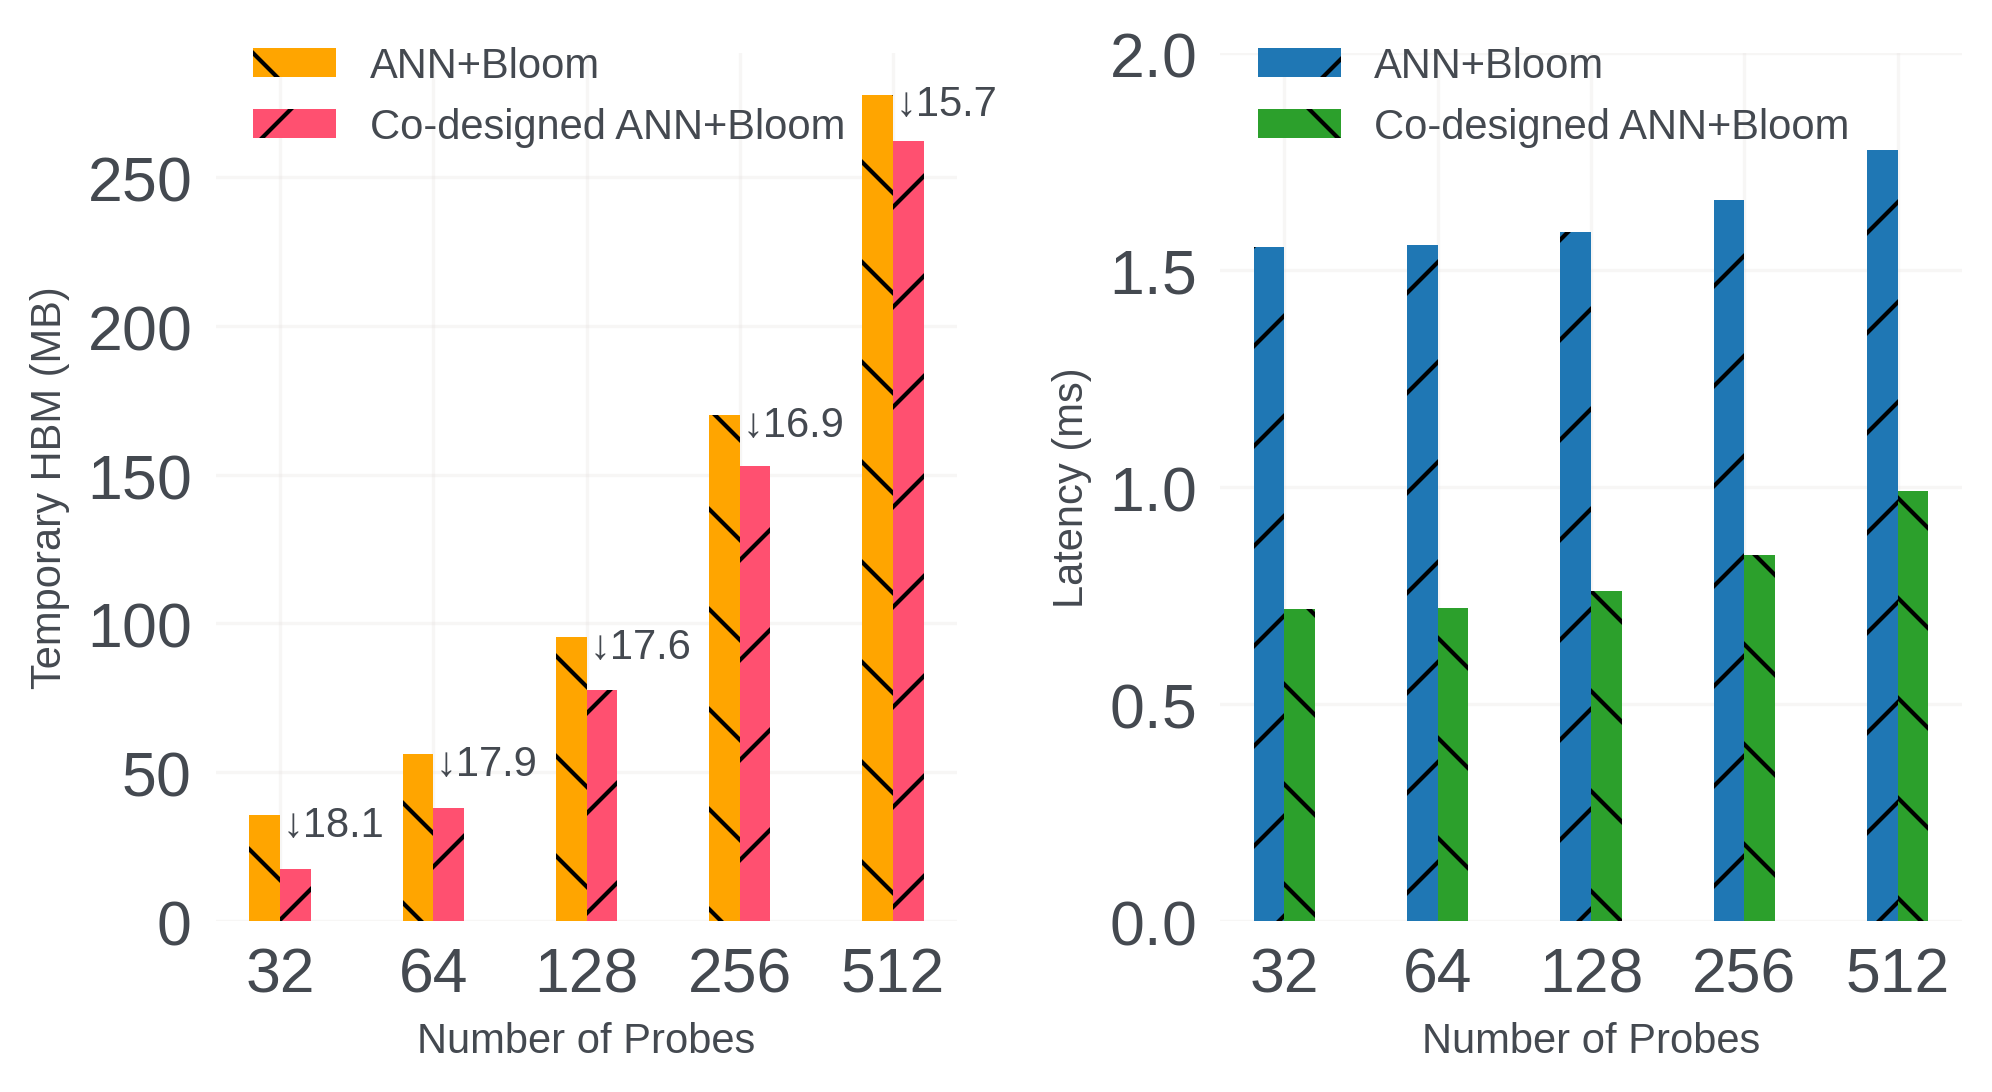
\includegraphics[width=0.95\textwidth]{fig11_codesigned_ann_bloom.png}
  \caption{Co-designing ANN search with Bloom filtering lowers temporary HBM usage and latency as the number of probes increases (Figure 11 in the paper).}
\end{figure}

\subsection*{Experiments}
\begin{itemize}[leftmargin=1.5em]
  \item \textbf{End-to-end retrieval at 80M scale.} With 24 probes (the paper's production setting), SilverTorch reaches \textbf{1210 QPS}, reported as \textbf{23.7$\times$} higher throughput than the CPU service baseline. At a 10-QPS send rate, average latency is about \textbf{14 ms}, a reported \textbf{11.4$\times$} reduction versus the CPU baseline.
  \item \textbf{Smaller-scale retrieval still benefits strongly.} On the 10M-item setup, SilverTorch reaches \textbf{3802 QPS}, reported as \textbf{165.3$\times$} above the unsharded CPU baseline and \textbf{20.8$\times$} above the GPU service baseline.
  \item \textbf{Cost efficiency.} Table 2 reports TCO/1000 requests of \$0.158 for the CPU baseline, \$0.0077 for SilverTorch, and \$0.012 for SilverTorch with OverArch+Value Model. That is \textbf{20.9$\times$} cost-efficiency improvement for base SilverTorch and \textbf{13.35$\times$} even after enabling the more accurate learned-scoring setup.
  \item \textbf{ESR embedding cache matters.} In early-stage ranking, the baseline times out above 5,720 items, while SilverTorch ranks up to \textbf{183,040} items. Around the 1k-item scale it achieves \textbf{4998 QPS} vs. \textbf{491} for the baseline (about \textbf{10.2$\times$} higher).
  \item \textbf{Component breakdowns support the design.} The Bloom Index is reported as \textbf{291--523$\times$} faster than the CPU inverted index and \textbf{12.6--42.7$\times$} faster than a GPU forward index, while using 2.4 GB at 1024 bits/item with only \textbf{0.06786\%} false positives. The co-designed ANN+Bloom path cuts a probe-32 example from \textbf{35.6 MB} scratch memory / \textbf{1.55 ms} latency to \textbf{18.2 MB} / \textbf{0.72 ms}. OverArch+Value Model increases E-Task Recall@20 from \textbf{0.07163} to \textbf{0.09181} (\textbf{+28.2\%}) while QPS drops from 1210 to 771, showing a deliberate quality/throughput tradeoff.
\end{itemize}

\subsection*{References (selected)}
\begin{itemize}[leftmargin=1.5em]
  \item Covington et al. (2016): deep neural networks for YouTube recommendations.
  \item Douze et al. (2024): the Faiss library.
  \item Wang et al. (2021): Milvus vector data management system.
  \item Borisyuk et al. (2024): LiNR, model-based neural retrieval on GPUs at LinkedIn.
  \item Ding \& Zhai (2025): retrieval with learned similarities / Mixture-of-Logits style scoring.
\end{itemize}

\end{document}
